% =====================================================================
%  Meeting deck for Šroubek + Harmanec
%  Focus: real-data training methodology + EquiUNet vs UNet results
%  Compile: pdflatex evaluation/presentation.tex (run twice for refs)
% =====================================================================
\documentclass[10pt,aspectratio=169]{beamer}
\usetheme{default}
\usecolortheme{seahorse}
\setbeamertemplate{navigation symbols}{}
\setbeamertemplate{footline}[frame number]

\usepackage[T1]{fontenc}
\usepackage{booktabs}
\usepackage{amsmath, amssymb}
\usepackage{graphicx}
\usepackage{array}
\usepackage{xcolor}
\usepackage{algorithmic}

\newcommand{\hilite}[1]{\textbf{\color{blue!60!black}#1}}

\title{Training EquiUNet vs UNet on real CCP data}
\subtitle{Methodology and results for the Shape2Fate detection backbone}
\author{Petr Vojtášek}
\date{\today}

\begin{document}

% =====================================================================
\begin{frame}[plain]
  \titlepage
\end{frame}

% =====================================================================
\begin{frame}{Outline}
  \begin{enumerate}\setlength\itemsep{3pt}
    \item Scope and dataset
    \item Mask examples --- what the network sees
    \item Multi-annotator fusion algorithms
    \item Equivariance motivation (synthetic capacity ablation)
    \item Training pipeline
    \item \hilite{Main results} --- merged-label training, fusion ablation
    \item Cross-annotator generalisation
    \item \hilite{Out-of-domain robustness} --- transfer to DYNAMIN/RPE
  \end{enumerate}
\end{frame}

% =====================================================================
\begin{frame}{Scope and dataset}
  \begin{block}{Question}
    For the Shape2Fate CCP detection backbone, does rotational equivariance
    pay off when training directly on real TIRF-SIM data?
  \end{block}

  \vspace{1mm}
  \centering
  \footnotesize
  \begin{tabular}{l l r r r}
    \toprule
    Stack & Role & Frames & Annotators & Pts/ann.\ (in ROI) \\
    \midrule
    \texttt{033} (RPE-1)     & train/val (80/20 contiguous) & 120 & 3 & 13.5\,k / 11.6\,k / 13.3\,k \\
    \texttt{012} (other cell) & held-out test                & 722 & 1 & 35.7\,k (438 tracks) \\
    \bottomrule
  \end{tabular}
  \normalsize

  \vspace{2mm}
  \begin{itemize}\setlength\itemsep{2pt}
    \item ROI: $[y\!=\!512{:}768,\,x\!=\!256{:}512]$, $256{\times}256$ px
    \item Per frame: $\sim$110--120 CCP per annotator
    \item Hyperparameters (lr, wd) inherited from synthetic-data hparam sweep
  \end{itemize}
\end{frame}

% =====================================================================
\begin{frame}{Mask examples --- what the network sees}
  \begin{columns}[T]
    \column{0.55\textwidth}
    \centering
    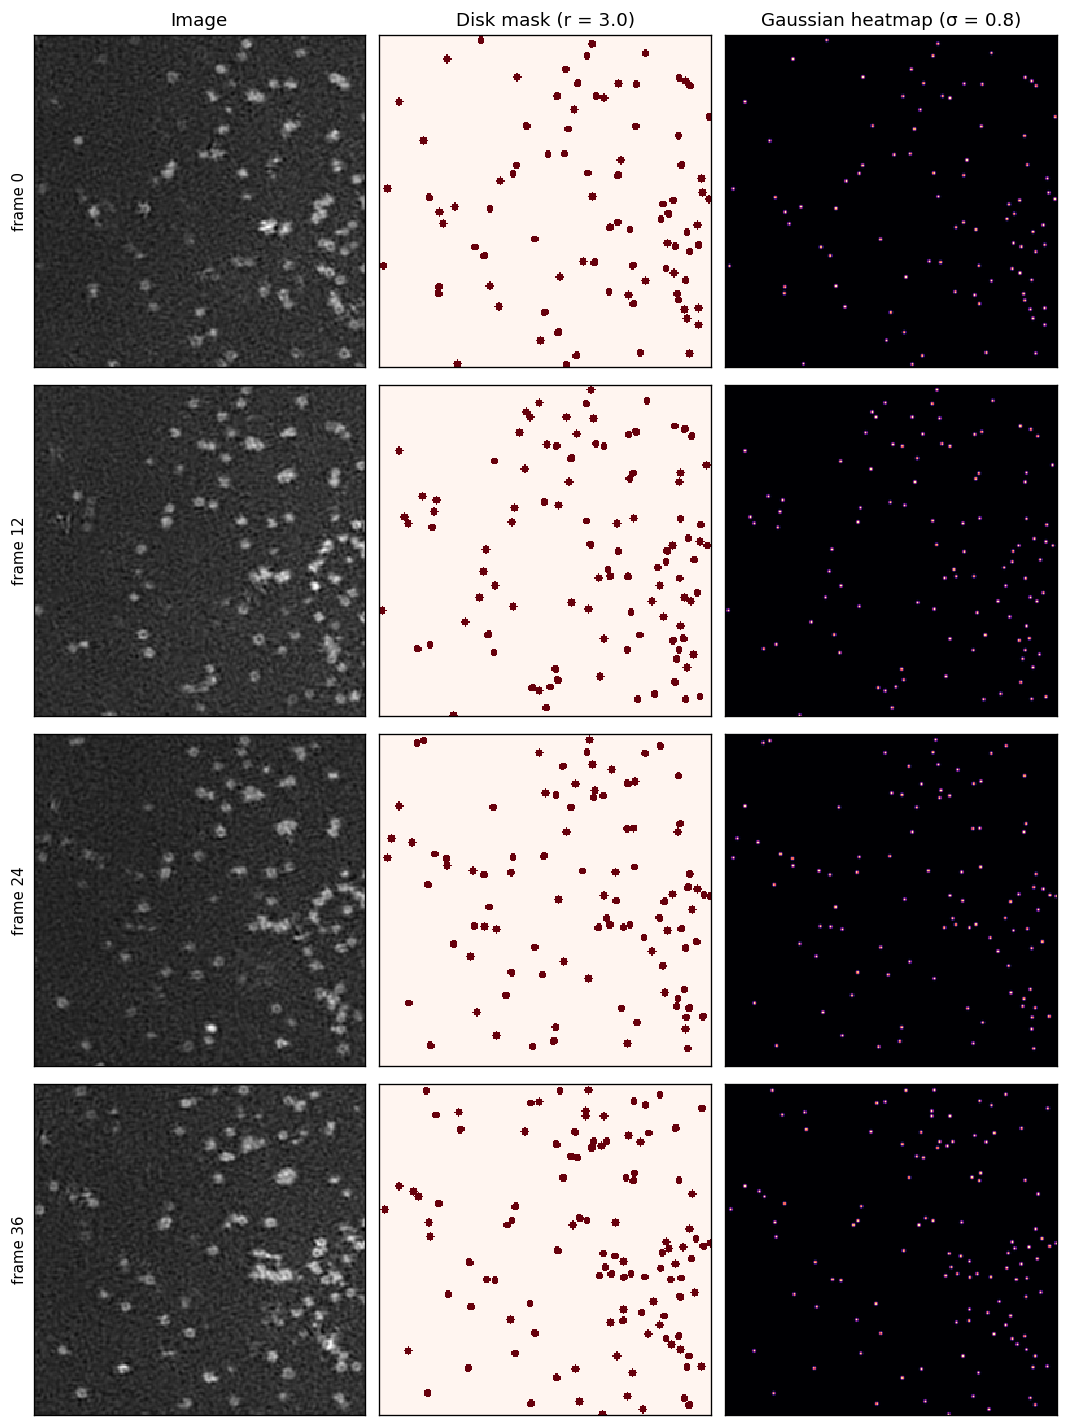
\includegraphics[height=0.82\textheight]{mask_examples.png}

    \column{0.45\textwidth}
    \footnotesize
    \textbf{Columns}
    \begin{itemize}\setlength\itemsep{0pt}
      \item raw SIM-reconstructed image (ROI crop)
      \item disk mask ($r{=}3$, alternative target)
      \item fused Gaussian mask ($\sigma{=}0.8$, training target)
    \end{itemize}

    \vspace{1mm}
    \textbf{Rows} --- 4 representative frames from the 033 val stack.

    \vspace{2mm}
    \textbf{Mask rendering}
    \[
      M(x, y) = \min\!\Bigl(\sum_{c \in \mathcal{C}}
        e^{-\tfrac{(x - c_x)^2 + (y - c_y)^2}{2\sigma^2}},\; 1\Bigr)
    \]
    Each fused centre $c \in \mathcal{C}$ contributes a Gaussian; sum clamped to keep the BCE target in $[0,1]$.
    \normalsize
  \end{columns}
\end{frame}

% =====================================================================
\begin{frame}{Multi-annotator fusion --- two algorithms compared}
  \begin{columns}[T]
    \column{0.5\textwidth}
    \textbf{Greedy (operational default)}
    \scriptsize
    \begin{algorithmic}[1]
      \REQUIRE pooled points $p_1, \dots, p_N$ in shuffled order; threshold $\tau$
      \STATE $\mathcal{K} \gets \emptyset$
      \FOR{each $p$}
        \IF{$\mathcal{K} = \emptyset$}
          \STATE start new cluster $\{p\}$
        \ELSE
          \STATE $j \gets \arg\min_{k} \| \bar{c}_k - p \|_2$
          \IF{$\| \bar{c}_j - p \|_2 < \tau$}
            \STATE append $p$ to cluster $j$, update $\bar{c}_j$
          \ELSE
            \STATE start new cluster $\{p\}$
          \ENDIF
        \ENDIF
      \ENDFOR
      \RETURN $\{\bar{c}_k\}$
    \end{algorithmic}
    \normalsize

    \column{0.5\textwidth}
    \textbf{Agglomerative complete-linkage}
    \scriptsize
    \begin{algorithmic}[1]
      \REQUIRE pooled points $P$; threshold $\tau$
      \STATE clusters $\gets \{\{p\} : p \in P\}$ \COMMENT{singletons}
      \LOOP
        \STATE $(A, B) \gets \arg\min_{X, Y} d_{\max}(X, Y)$
        \STATE \hspace{4mm} where $d_{\max}(X,Y) = \max_{a \in X, b \in Y} \|a-b\|_2$
        \IF{$d_{\max}(A, B) < \tau$}
          \STATE merge $A$ and $B$
        \ELSE
          \STATE \textbf{stop}
        \ENDIF
      \ENDLOOP
      \RETURN cluster centroids
    \end{algorithmic}
    \normalsize
  \end{columns}

  \vspace{1mm}
  \centering
  \scriptsize
  \begin{tabular}{l l l l}
    \toprule
    & order-dependent? & complexity & cluster diameter \\
    \midrule
    Greedy           & yes (shuffled per-frame, seed = frame) & $\mathcal{O}(NK)$         & may exceed $\tau$ (chain merge) \\
    Complete-linkage & no                                     & $\mathcal{O}(N^2 \log N)$ & $\leq \tau$ by construction      \\
    \bottomrule
  \end{tabular}
\end{frame}

% =====================================================================
\begin{frame}{Equivariance motivation --- synthetic capacity ablation}
  \centering
  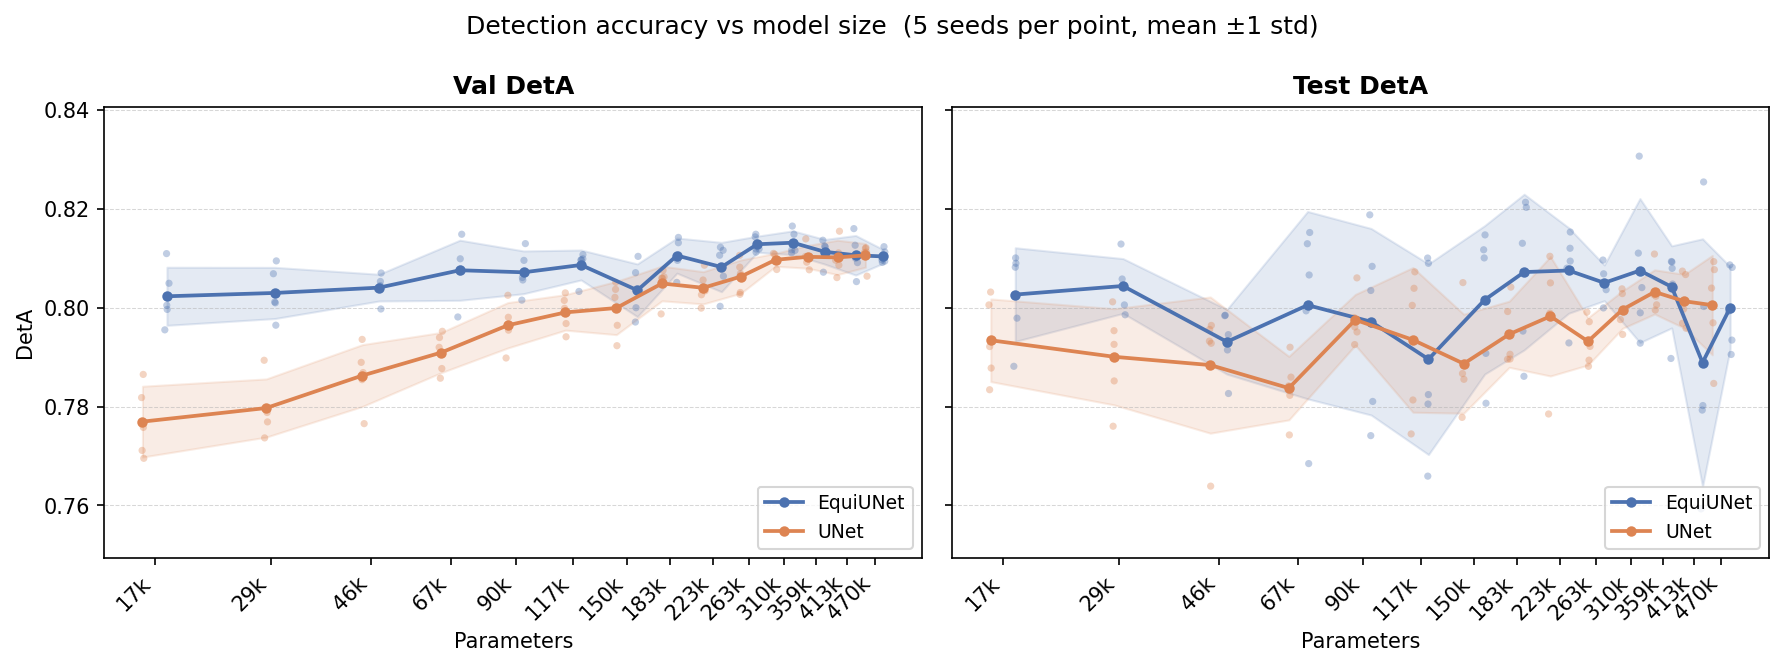
\includegraphics[width=0.88\textwidth]{deta_by_start_filters.png}

  \vspace{0mm}
  \footnotesize 5 seeds per point, mean $\pm$ 1 std. Val/test on real CCP frames.
  \normalsize

  \begin{itemize}\setlength\itemsep{0pt}\footnotesize
    \item EquiUNet leads by $\sim +0.03$ DetA at $\sim$17\,k params $\Rightarrow$
          equivariance as a \hilite{parameter-efficient prior}
    \item Both saturate at $\sim 0.81$ from $\sim$110\,k params $\Rightarrow$
          \hilite{data/label-noise ceiling, not capacity}
    \item Does the benefit hold when \emph{training directly on real data}?
  \end{itemize}
\end{frame}

% =====================================================================
\begin{frame}{Training pipeline}
  \centering
  \footnotesize
  \begin{tabular}{l l l}
    \toprule
                              & \textbf{UNet}            & \textbf{EquiUNet}                \\
    \midrule
    start filters / depth     & 16 / 3                   & 16 / 3                           \\
    parameters                & $\approx 450$\,k         & $\approx 489$\,k                 \\
    symmetry group            & ---                      & $\mathrm{SO}(2)$, fourierbn act. \\
    conv kernel               & $3 \times 3$             & $5 \times 5$                     \\
    learning rate             & $1.6 \cdot 10^{-4}$      & $4.7 \cdot 10^{-3}$              \\
    weight decay              & $0.05$                   & $0.082$                          \\
    \midrule
    \multicolumn{3}{l}{shared schedule: AdamW, BCE loss, 100 epochs, batch 16,
                       $128 {\times} 128$ patches, val every epoch, 5 seeds} \\
    \bottomrule
  \end{tabular}
  \normalsize

  \vspace{3mm}
  \begin{itemize}\setlength\itemsep{1pt}
    \item Inference: full $1024 \times 1024$ frame in one forward pass
          (fully convolutional), peak-finding, ROI filter post-hoc
  \end{itemize}
\end{frame}

% =====================================================================
\begin{frame}{Main result --- UNet vs EquiUNet on merged real labels}
  \centering
  \begin{tabular}{l c c}
    \toprule
    Model                       & Val DetA                 & Test DetA \\
    \midrule
    UNet sf=16                  & $0.7783 \pm 0.0118$      & $0.8071 \pm 0.0218$ \\
    \hilite{EquiUNet sf=16}     & \hilite{$0.7831 \pm 0.0059$} & \hilite{$0.8116 \pm 0.0150$} \\
    \midrule
    $\Delta$ (Equi $-$ UNet)    & $+0.0048$                & $+0.0045$ \\
    Welch $p$                   & $0.45$ \textit{(n.s.)}   & $0.72$ \textit{(n.s.)} \\
    \bottomrule
  \end{tabular}

  \vspace{3mm}
  \begin{itemize}\setlength\itemsep{2pt}
    \item Point estimate equi leads, but \hilite{within seed noise at $n=5$}
    \item \hilite{Seed std $\sim 2{\times}$ smaller for EquiUNet}
          $\Rightarrow$ symmetry stabilises optimisation
    \item Equivariance becomes statistically significant under noisier-mask
          conditions (fusion ablation, next slide)
  \end{itemize}
\end{frame}

% =====================================================================
\begin{frame}{Fusion-algorithm ablation --- architecture robustness}
  5 seeds per cell, val DetA.

  \vspace{2mm}
  \centering
  \footnotesize
  \begin{tabular}{l c c c}
    \toprule
                                 & Greedy $\tau{=}5$       & Complete $\tau{=}5$     & Complete $\tau{=}4$     \\
    \midrule
    UNet                         & $0.7783 \pm 0.0118$    & $0.7620 \pm 0.0127$     & $0.7463 \pm 0.0069$     \\
    EquiUNet                     & $0.7831 \pm 0.0059$    & \hilite{$0.7855 \pm 0.0040$} & $0.7685 \pm 0.0065$ \\
    \midrule
    Welch $p$ (Equi $-$ UNet)    & $0.45$ \textit{(n.s.)} & \hilite{$0.012\,^{*}$}  & \hilite{$<\!0.001\,^{***}$} \\
    \bottomrule
  \end{tabular}
  \normalsize

  \vspace{3mm}
  \centering
  \footnotesize
  \begin{tabular}{l c}
    \toprule
    Within-architecture comparison                            & Welch $p$ \\
    \midrule
    UNet: greedy $\to$ complete-linkage (both $\tau{=}5$)       & $0.069$ \quad (marginal) \\
    EquiUNet: greedy $\to$ complete-linkage (both $\tau{=}5$)   & $0.48$ \quad \textit{(n.s.)} \\
    UNet: $\tau{=}5 \to \tau{=}4$ (complete-linkage)            & $0.051$ \quad (marginal) \\
    EquiUNet: $\tau{=}5 \to \tau{=}4$ (complete-linkage)        & $0.002\,^{**}$ \\
    \bottomrule
  \end{tabular}
  \normalsize

  \vspace{2mm}
  \footnotesize \hilite{Equivariance prior absorbs the algorithm choice}; the
  threshold remains a universal lever.
\end{frame}

% =====================================================================
\begin{frame}{Cross-annotator generalisation --- per-direction breakdown}
  Same training pipeline, but mask = single annotator (no fusion), val DetA scored
  per held-out annotator. 5 seeds $\times$ 3 train annotators = 15 runs / architecture.

  \vspace{2mm}
  \centering
  \scriptsize
  \begin{tabular}{c c c c c c c}
    \toprule
    train     & eval      & IAA (humans) & UNet                  & $\Delta$ vs IAA & EquiUNet              & $\Delta$ vs IAA \\
    \midrule
    ann1      & ann2      & $0.740$ & $0.693 \pm 0.016$           & $-0.047$        & $0.718 \pm 0.009$     & $-0.022$        \\
    ann1      & ann3      & $0.748$ & $0.752 \pm 0.013$           & $+0.003$        & $0.770 \pm 0.011$     & $+0.022$        \\
    \multicolumn{2}{r}{\emph{ann1 $\to$}} & $0.744$ & $0.723$ & $-0.022$ & $0.744$ & $0.000$ \\
    \midrule
    \hilite{ann2} & \hilite{ann1} & $0.740$ & \hilite{$0.842 \pm 0.014$} & \hilite{$+0.102$} & \hilite{$0.851 \pm 0.010$} & \hilite{$+0.111$} \\
    ann2      & ann3      & $0.730$ & $0.777 \pm 0.023$           & $+0.047$        & $0.782 \pm 0.004$     & $+0.052$        \\
    \multicolumn{2}{r}{\emph{ann2 $\to$}} & $0.735$ & \hilite{$0.810$} & \hilite{$+0.075$} & \hilite{$0.817$} & \hilite{$+0.082$} \\
    \midrule
    \hilite{ann3} & \hilite{ann1} & $0.748$ & \hilite{$0.845 \pm 0.007$} & \hilite{$+0.096$} & $0.839 \pm 0.016$ & $+0.091$        \\
    ann3      & ann2      & $0.730$ & $0.705 \pm 0.015$           & $-0.025$        & $0.721 \pm 0.018$     & $-0.009$        \\
    \multicolumn{2}{r}{\emph{ann3 $\to$}} & $0.739$ & $0.775$ & $+0.036$ & $0.780$ & $+0.041$ \\
    \midrule
    \multicolumn{2}{r}{\emph{global aggregate}} & $0.7393$ & $0.7688 \pm 0.0394$ & $+0.0295$ & \hilite{$0.7802 \pm 0.0316$} & \hilite{$+0.0409$} \\
    \bottomrule
  \end{tabular}
  \normalsize

  \vspace{2mm}
  \begin{itemize}\setlength\itemsep{1pt}
    \item \hilite{Networks exceed the human inter-annotator ceiling} in 4/6 directions
          $\Rightarrow$ network acts as a \emph{label denoiser}
    \item Predicting ann2 (strict outlier, 11.6\,k pts) is the only direction where
          networks underperform IAA; EquiUNet shrinks the gap
  \end{itemize}
\end{frame}

% =====================================================================
\begin{frame}{Out-of-domain robustness --- transfer to DYNAMIN/RPE}
  \small
  Test stack disjoint from training (RPE1-egfpCLCa 033 $\rightarrow$ DYNAMIN/RPE 195), 151 frames, full HOTA pipeline. 5 seeds per config.
  \normalsize

  \vspace{3mm}
  \centering
  \footnotesize
  \begin{tabular}{l c c}
    \toprule
    Config            & HOTA                       & DetA                       \\
    \midrule
    \hilite{Synth UNet}     & \hilite{$0.777 \pm 0.013$} & \hilite{$0.856 \pm 0.011$} \\
    Synth EquiUNet          & $0.760 \pm 0.019$          & $0.839 \pm 0.018$          \\
    Real EquiUNet           & $0.650 \pm 0.025$          & $0.700 \pm 0.029$          \\
    Real UNet               & $0.617 \pm 0.047$          & $0.644 \pm 0.055$          \\
    \bottomrule
  \end{tabular}

  \vspace{4mm}
  \centering
  \footnotesize
  \begin{tabular}{l c c}
    \toprule
    Welch $t$-test (DetA)                  & $\Delta$    & $p$               \\
    \midrule
    Synth UNet \;\;vs\;\; Real UNet        & $+0.212$    & $0.0008$\,***     \\
    Synth EquiUNet vs Real EquiUNet        & $+0.139$    & $<\!0.0001$\,***  \\
    Synth UNet \;\;vs\;\; Synth EquiUNet   & $+0.017$    & $0.11$ \textit{(n.s.)} \\
    \bottomrule
  \end{tabular}
  \normalsize

  \vspace{3mm}
  \small \hilite{Synth UNet wins.} Synthetic training generalises to OOD data;
  equivariance prior brings no benefit once the training distribution is diverse.
\end{frame}

% =====================================================================
\begin{frame}{Summary}
  \begin{enumerate}\setlength\itemsep{4pt}
    \item Real-data training pipeline for the Shape2Fate detection backbone:
          3-annotator greedy fusion ($\tau{=}5$, deterministic shuffle),
          Gaussian mask $\sigma{=}0.8$, BCE loss.
    \item On merged labels (5 seeds, greedy $\tau{=}5$): EquiUNet point estimate
          leads UNet, but \hilite{$+0.005$ val DetA is within seed noise
          (Welch $p = 0.45$)}; seed std $\sim 2 \times$ smaller for EquiUNet.
    \item Fusion-algorithm ablation: \hilite{equivariance is statistically robust
          to upstream label noise}; complete-linkage gives EquiUNet $+0.024$
          over UNet (Welch $p \leq 0.012$).
    \item Cross-annotator: networks \hilite{exceed human inter-annotator
          agreement} (0.78 vs 0.74 IAA) --- network as label denoiser.
    \item \hilite{Out-of-domain robustness (DYNAMIN/RPE):} synthetic-trained
          models beat real-trained by $+0.14$ to $+0.21$ DetA ($p \leq 0.001$);
          architecture irrelevant within synth ($p = 0.11$).
  \end{enumerate}
\end{frame}

\end{document}
